\documentclass{article}
\usepackage{amsmath}
\usepackage{tikz}
\usetikzlibrary{positioning}

\begin{document}

\begin{align*}
-2\eta &\leq r - d(x,y) \leq -g'(-\eta) \\
&\quad x \overset{\phi_s g'}{\longrightarrow} g'(\eta) 
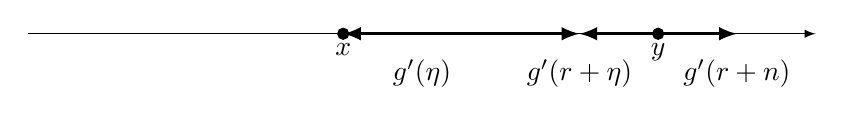
\begin{tikzpicture}[baseline=(current bounding box.center),>=latex]
    \draw[->] (-1,0) -- (9,0);
    \filldraw[black] (3,0) circle (2pt) node[below] {$x$};
    \filldraw[black] (7,0) circle (2pt) node[below] {$y$};
    \node at (4,-0.5) {$g'(\eta)$};
    \node at (6,-0.5) {$g'(r+\eta)$};
    \node at (8,-0.5) {$g'(r+n)$};
    \draw[<->,very thick] (3,0) -- (6,0);
    \draw[<->,very thick] (6,0) -- (8,0);
\end{tikzpicture} \\
-\eta &\leq r - d(x,y) \leq 0 \\
&\quad x \overset{\phi_s g'}{\longrightarrow} g'(\eta) 
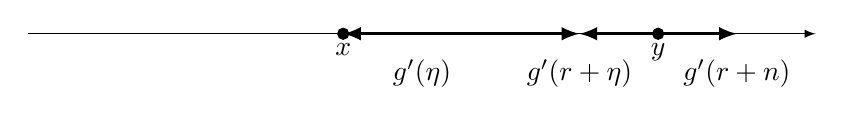
\begin{tikzpicture}[baseline=(current bounding box.center),>=latex]
    \draw[->] (-1,0) -- (9,0);
    \filldraw[black] (3,0) circle (2pt) node[below] {$x$};
    \filldraw[black] (7,0) circle (2pt) node[below] {$y$};
    \node at (4,-0.5) {$g'(\eta)$};
    \node at (6,-0.5) {$g'(r+\eta)$};
    \node at (8,-0.5) {$g'(r+n)$};
    \draw[<->,very thick] (3,0) -- (6,0);
    \draw[<->,very thick] (6,0) -- (8,0);
\end{tikzpicture} \\
0 &\leq r - d(x,y) \leq \eta \\
&\quad x \overset{\phi_s g'}{\longrightarrow} g'(\eta) 
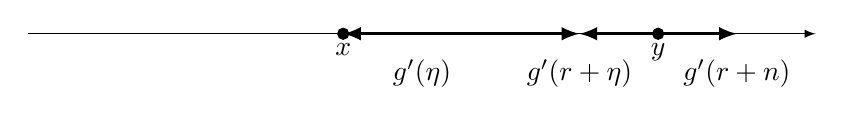
\begin{tikzpicture}[baseline=(current bounding box.center),>=latex]
    \draw[->] (-1,0) -- (9,0);
    \filldraw[black] (3,0) circle (2pt) node[below] {$x$};
    \filldraw[black] (7,0) circle (2pt) node[below] {$y$};
    \node at (4,-0.5) {$g'(\eta)$};
    \node at (6,-0.5) {$g'(r+\eta)$};
    \node at (8,-0.5) {$g'(r+n)$};
    \draw[<->,very thick] (3,0) -- (6,0);
    \draw[<->,very thick] (6,0) -- (8,0);
\end{tikzpicture} \\
\eta &\leq r - d(x,y) \leq 2\eta \\
&\quad x \overset{\phi_s g'}{\longrightarrow} g(\eta) 
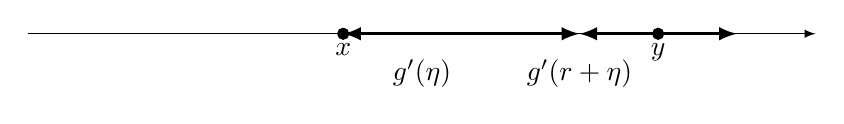
\begin{tikzpicture}[baseline=(current bounding box.center),>=latex]
    \draw[->] (-1,0) -- (9,0);
    \filldraw[black] (3,0) circle (2pt) node[below] {$x$};
    \filldraw[black] (7,0) circle (2pt) node[below] {$y$};
    \node at (4,-0.5) {$g'(\eta)$};
    \node at (6,-0.5) {$g'(r+\eta)$};
    \draw[<->,very thick] (3,0) -- (6,0);
    \draw[<->,very thick] (6,0) -- (8,0);
\end{tikzpicture}
\end{align*}

\end{document}